%
% File acl2018.tex
%
%% Based on the style files for ACL-2017, with some changes, which were, in turn,
%% Based on the style files for ACL-2015, with some improvements
%%  taken from the NAACL-2016 style
%% Based on the style files for ACL-2014, which were, in turn,
%% based on ACL-2013, ACL-2012, ACL-2011, ACL-2010, ACL-IJCNLP-2009,
%% EACL-2009, IJCNLP-2008...
%% Based on the style files for EACL 2006 by 
%%e.agirre@ehu.es or Sergi.Balari@uab.es
%% and that of ACL 08 by Joakim Nivre and Noah Smith

\documentclass[11pt,a4paper]{article}
\usepackage[hyperref]{acl2018}
\usepackage{times}
\usepackage{latexsym}
\usepackage{amsmath}
\usepackage{url}

\usepackage{tabularx}

\usepackage{graphicx}
\graphicspath{ {graphics/} }

\aclfinalcopy % Uncomment this line for the final submission
%\def\aclpaperid{***} %  Enter the acl Paper ID here

%\setlength\titlebox{5cm}
% You can expand the titlebox if you need extra space
% to show all the authors. Please do not make the titlebox
% smaller than 5cm (the original size); we will check this
% in the camera-ready version and ask you to change it back.

\newcommand\BibTeX{B{\sc ib}\TeX}

\title{Spoken Language Understanding Module for Movie Domain \\ Mid-term project}

\author{Andrea Tupini \\
  MAT.  194578 \\
  {\tt andrea.tupini@studenti.unitn.it}}

\date{}

\begin{document}
	
\maketitle

\begin{abstract}
	
	In this work we build a simple tagger that predicts the IOB tags of words in a sentence. The tagger will be an WFST (weighted finite state machine) model composed with an n-gram model. We'll compare its performance when building it with different smoothing methods and n-gram lengths, and see a very simple change we can do to the data that increases the overral performance of the model. 
	\\
	
\end{abstract}

\section{Introduction}

	A concept tagger is an important part in any SLU pipeline since it lets us tag each input word with the proper tag that tells the rest of the system how to process said word and the ones near it. In the specific system we'll be building the tagger tells us if a word is one of a number of tags about the movie domain (name of a movie, actor, etc) or something else. The tags we'll be working with are in IOB notation, which will be explained a bit in section 6\ref{sec-data-analysis}. 
	
	This work will be mainly dedicated to constructing and comparing the performance of predicting the correct IOB tags with 2 different models. One uses just a plain word to IOB tag transducer plus an n-gram model of the IOB tags in the train set to predict the correct tags of a test sentence, and the other is practically the same except that we try countering the fact that O tags don't offer us much information. A more detailed explanation of the models will be given in the next section.
	

\section{Models}

	We want to create a model that, given a sequence of words $w_1, ... , w_n$ finds the most probable tag sequence $t_1, ... , t_n$ where:
	
	$$
	t_1, ... , t_n = \operatorname*{argmax}_{t_1,...,t_n} P(t_1,...,t_n | w_1,...,w_n)
	$$
	
	If we apply Bayes's theorem, and take the following simplifications:
	
	\begin{itemize}
		\item We can remove the denominator (evidence) since it doesn't depend on $t_1,...,t_n$
		\item The probability of a word only depends on its own tag (and not the tags of other words)
		\item The probability of the tags also depends on the tags near it up to a certain degree (n-gram part of the model)
	\end{itemize}
	
	We get that:
	
	$$
	 t_1, ... , t_n = \operatorname*{argmax}_{t_1,...,t_n} 
	 \prod_{i=1}^{n} P(w_i | t_i) P(t_i | t_{i-1})
	$$

	where \textit{i} denotes the \textit{i'th} word. Here is a breakdown of the model:
	
	\begin{description}
		\item[$P(w_i|t_i)$] Is the probability of seeing current word given tag
		\item[$P(t_i|t_{i-1})$] Is the probability of seeing current tag given previous tag (note that this is for a bigram model, but we can consider extra, previous tags, to generalize for any n-gram)
	\end{description}
	
	To calculate these terms we use the following. Note that since we want to treat $P(w_i|t_i)$ as a score we pass also pass it through a $-log$:
	
	$$
	P(w_i|t_i) = -\log \frac{C(t_i, w_i)}{C(t_i)}
	$$
	$$
	P(t_i|t_{i-1}) = \frac{C(t_{i-1}, t_i)}{C(t_{i-1})}
	$$
	
	For unknown words the $P(w_i|t_i)$ term gets calculated a bit differently. An unknown word can be tagged with any tag, with equal possibility:
	
	$$
	P(<unk>|t_i) = \frac{1}{C(t)}
	$$
	
	So, a transition is added from an unknown keyword to a tag $t_i$ and the probability of said transition is $\frac{1}{total\ amount\ of\ tags}$.
	
	Based on these assumptions, the following three models were produced to predict the IOB tag of a word in a sentence:
	
	\begin{description}
		\item[Baseline] The baseline model is the most basic model possible and is the one against which we evaluate the performance of the other two models. For the baseline model we consider a \textbf{unigram} model with \textbf{no smoothing}
		\item[Basic
		 Model] This model uses the training set as it is, and is trained to produce IOB tags. 
		\item[Improved Model] The improved model is trained on a modified version of the training set: all \textit{O} tags are replaced by \textit{O\_\_word}. 
	\end{description}

	For creating the models we use the \textit{OpenFst} \cite{openfst} and \textit{OpenGrm} \cite{opengrm} libraries, which give us helping functions for creating and managing n-gram models and transducers.

	When building the \textit{IOB Model} and \textit{Improved Model} we dynamically find what is the best combination of \textit{n-gram lengths} and \textit{smoothing method}. We only consider n-gram lengths from 1 to 5 (inclusive) and the smoothing methods that are supported by the \textit{OpenGrm} library (which are \textit{absolute, katz, kneser ney, presmoothed, unsmoothed and witten bell}).
	
\section{Data Analysis}
\label{sec-data-analysis}

	The provided data is composed of 4 different files in \textit{NL-SPARQL} format. These are composed of multiple sentences and each word in each sentence is tagged with its IOB tag, POS tag and lemma. Said files are:
	
	\begin{description}
		\item[NLSPARQL.test] words and IOB tags for testing
		\item[NLSPARQL.train] words and IOB tags for training              
		\item[NLSPARQL.test.feats] words, POS tags and lemmas for testing
		\item[NLSPARQL.train.feats] words, POS tags and lemmas for training
	\end{description}

	The models we'll develop will use the \textit{test} and \textit{train} files, but we'll also briefly visit the \textit{train.feats} file to see the distribution of POS tags in the data.
	
	As said above, the data we'll use is composed of words and IOB tags. IOB tags (Inside-Outside-Beginning) use the concept of span, which lets us know when a word marks the beginning of a concept (tag B), when it is a word inside of a concept (tag I) and when the word is simply outside of the concept (O). Besides this, the tag also tells us what the concept is about: movie name, actor, etc (all tags relating to the movie domain). Following is an example of what a sentence looks like in the dataset:
	
	\begin{table}[h]
		\begin{tabularx}{198pt}{l | l}
			\centering
	 	 	\textbf{Word} & \textbf{Tag} \\
			\hline 
			who & O \\
			plays & O \\
			luke & B-character.name \\
			on & O \\
			star & B-movie.name \\
			wars & I-movie.name \\
			new & I-movie.name \\
			hope & I-movie.name \\
 		\end{tabularx} 
		\caption{Example sentence in train set}
		\label{table:example-sentence}	
	\end{table}

	
	In the data we have a total of \textit{41} different tags, one of which is just the O tag, and the rest are \textit{20} matching B and I tags. Following is a bar plot of the tags ordered by their counts, note that the counts are scaled with \textit{log} so it's easier to see the value of other tags besides the O:
	
	\hspace*{-0.9cm}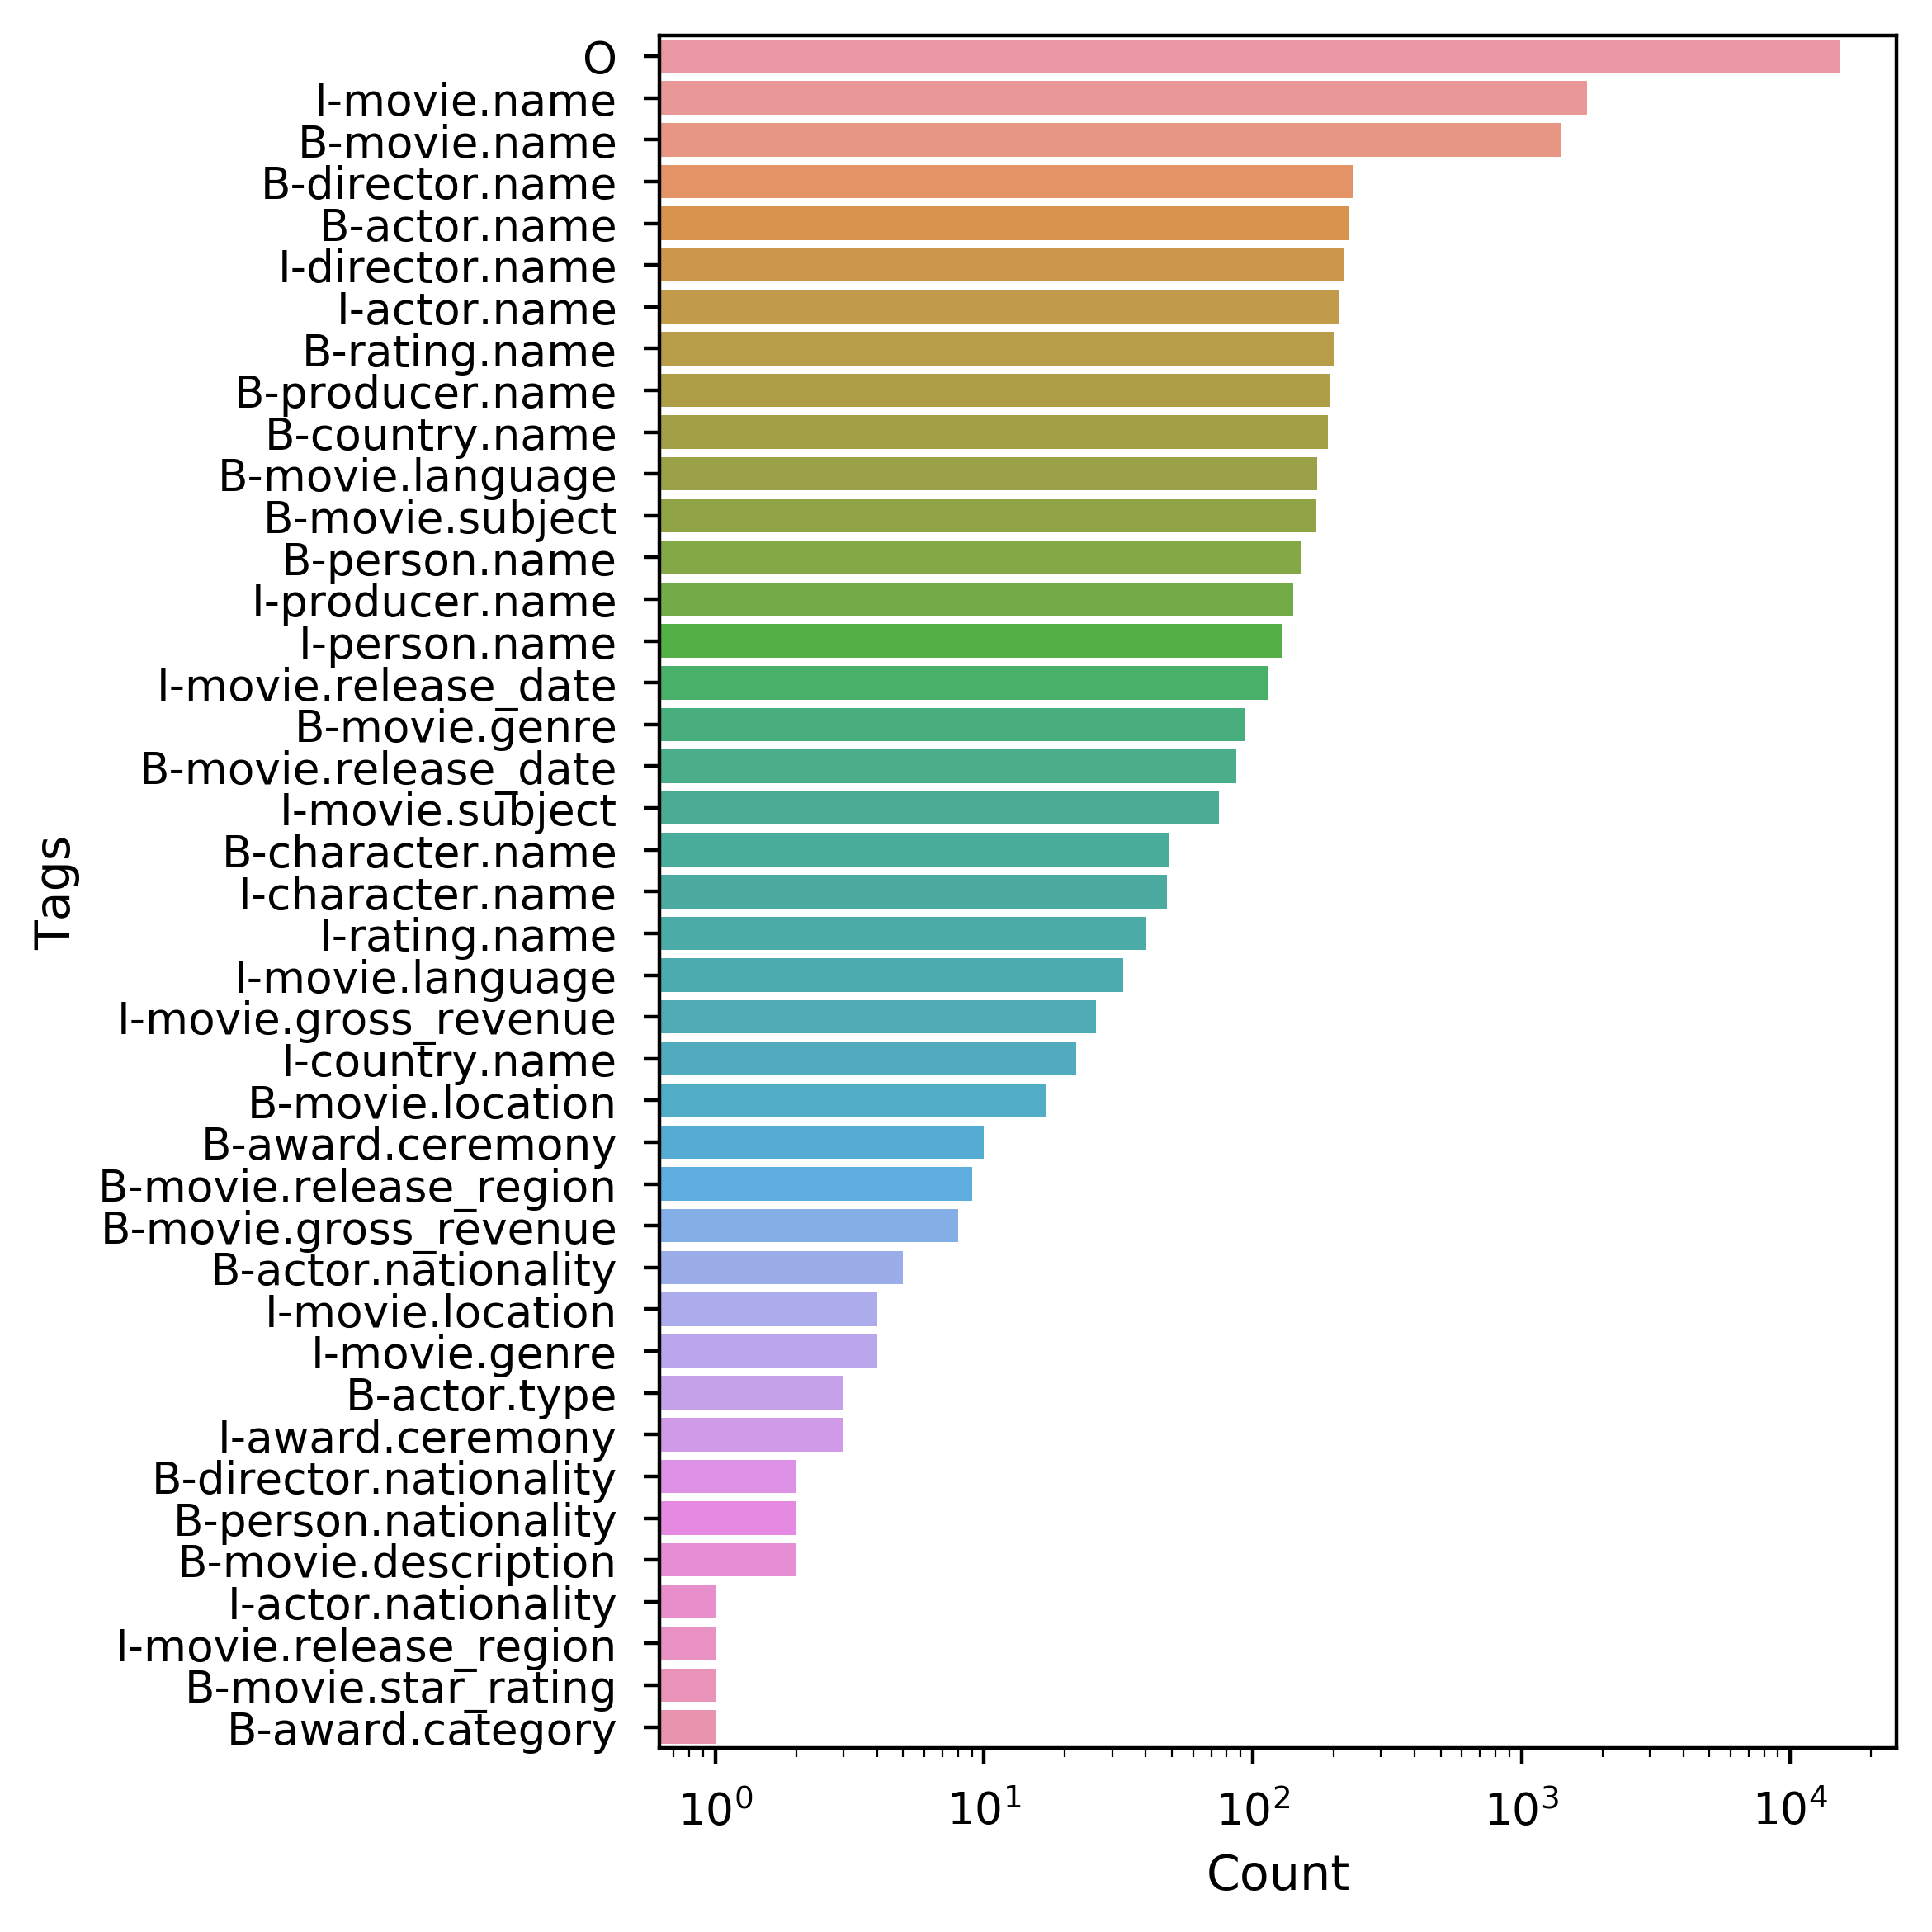
\includegraphics[scale=0.5]{barplot_iob_tag_counts}

	As we can see, the great majority of tags is simply O. In the training data there are a total of \textit{21453} tagged words, of which \textit{15391} are O tags, that is the \textit{71.74}\% of all tags. This is because most of the words are just filler words that link a concept with another or are words that say what is wanted but don't represent a concept per se. This makes sense but it will be a bit of a problem when we're "training" our tagger, since O's don't tell us much about the word itself and a word can appear multiple times and can be tagged with either O, B or I tags, introducing possible errors. In fact, the only difference between the normal model and the improved one is that in the improved model the O's get replaced by \textit{O\_\_word} so that we preserve the word's information in the tag. As we'll see later, this simple change notably improves the performance of the model. 
	
	As for the sentences per se, they're queries like the example sentence presented in \textit{Table \ref{table:example-sentence}} which ask some information about the movie domain. There are a total of \textit{1728} distinct words in the training set, following we can see a bar plot of the 30 most common words and their counts:

	\hspace*{-0.9cm}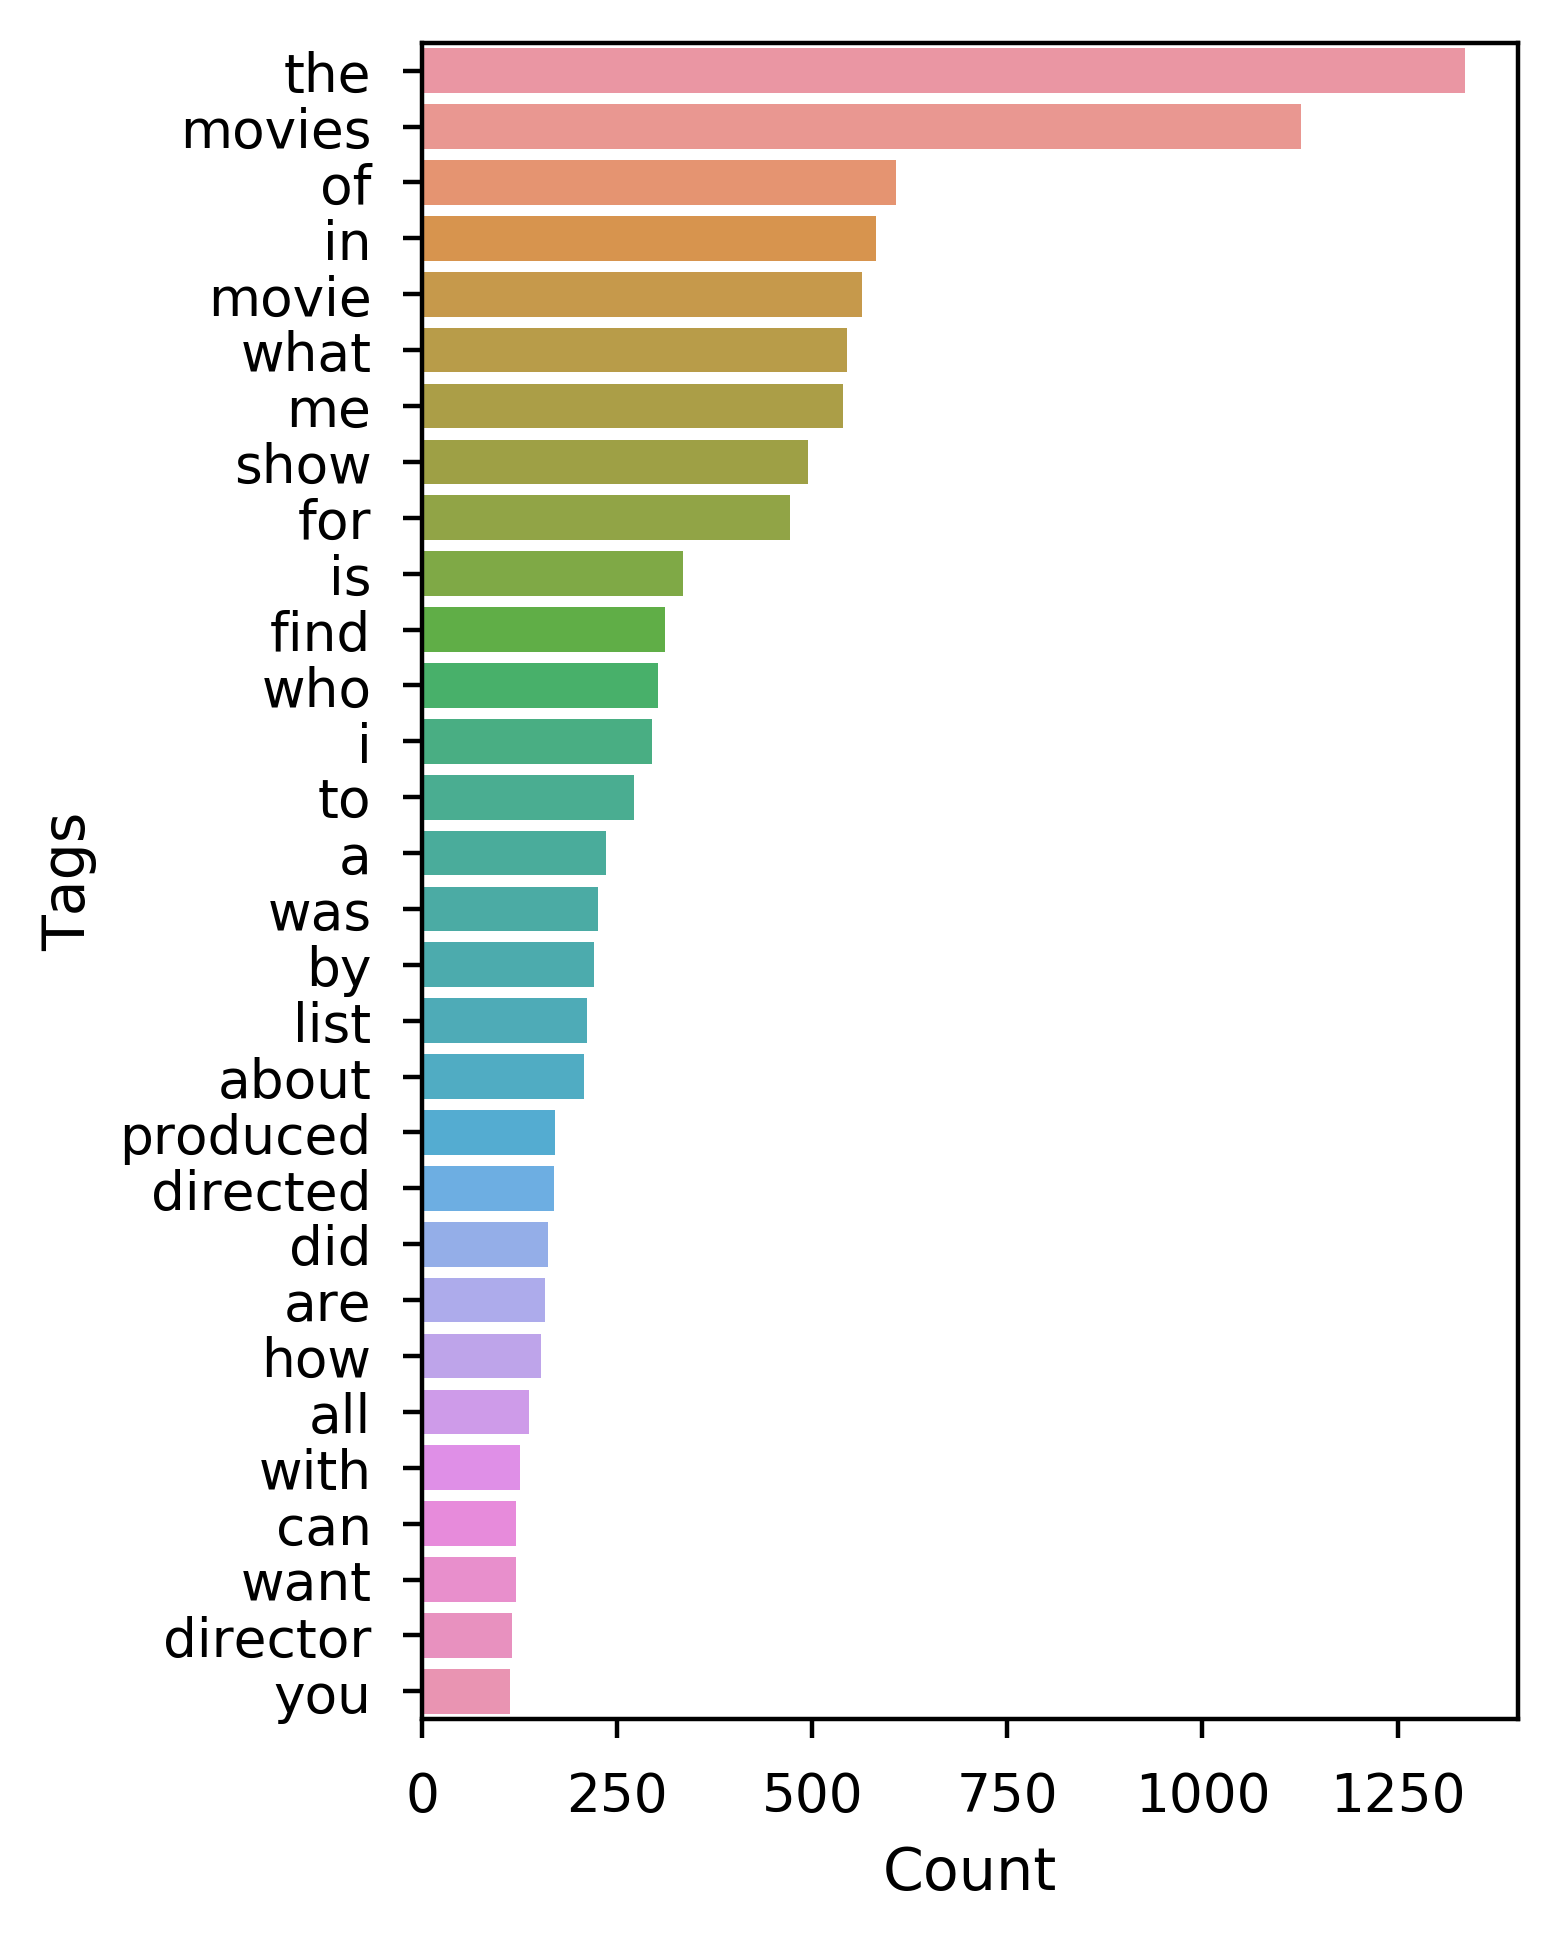
\includegraphics[scale=0.7]{barplot_iob&w_tag_counts_onlyW}
	
	As expected, the list of most common words is a composition between stopwords (the, of, in, is, a, etc), move domain specific words (movies, movie, show, director, etc) and words that represent a query (who, find, show, how, etc). We can see that the words \textit{the} and \textit{movies} appear quite a bit more times than any other word in the set.
	
	As mentioned above, we also have access to the POS tags of each word. Below we can see a bar plot which shows all of the POS tags and their counts:

	\hspace*{-0.7cm}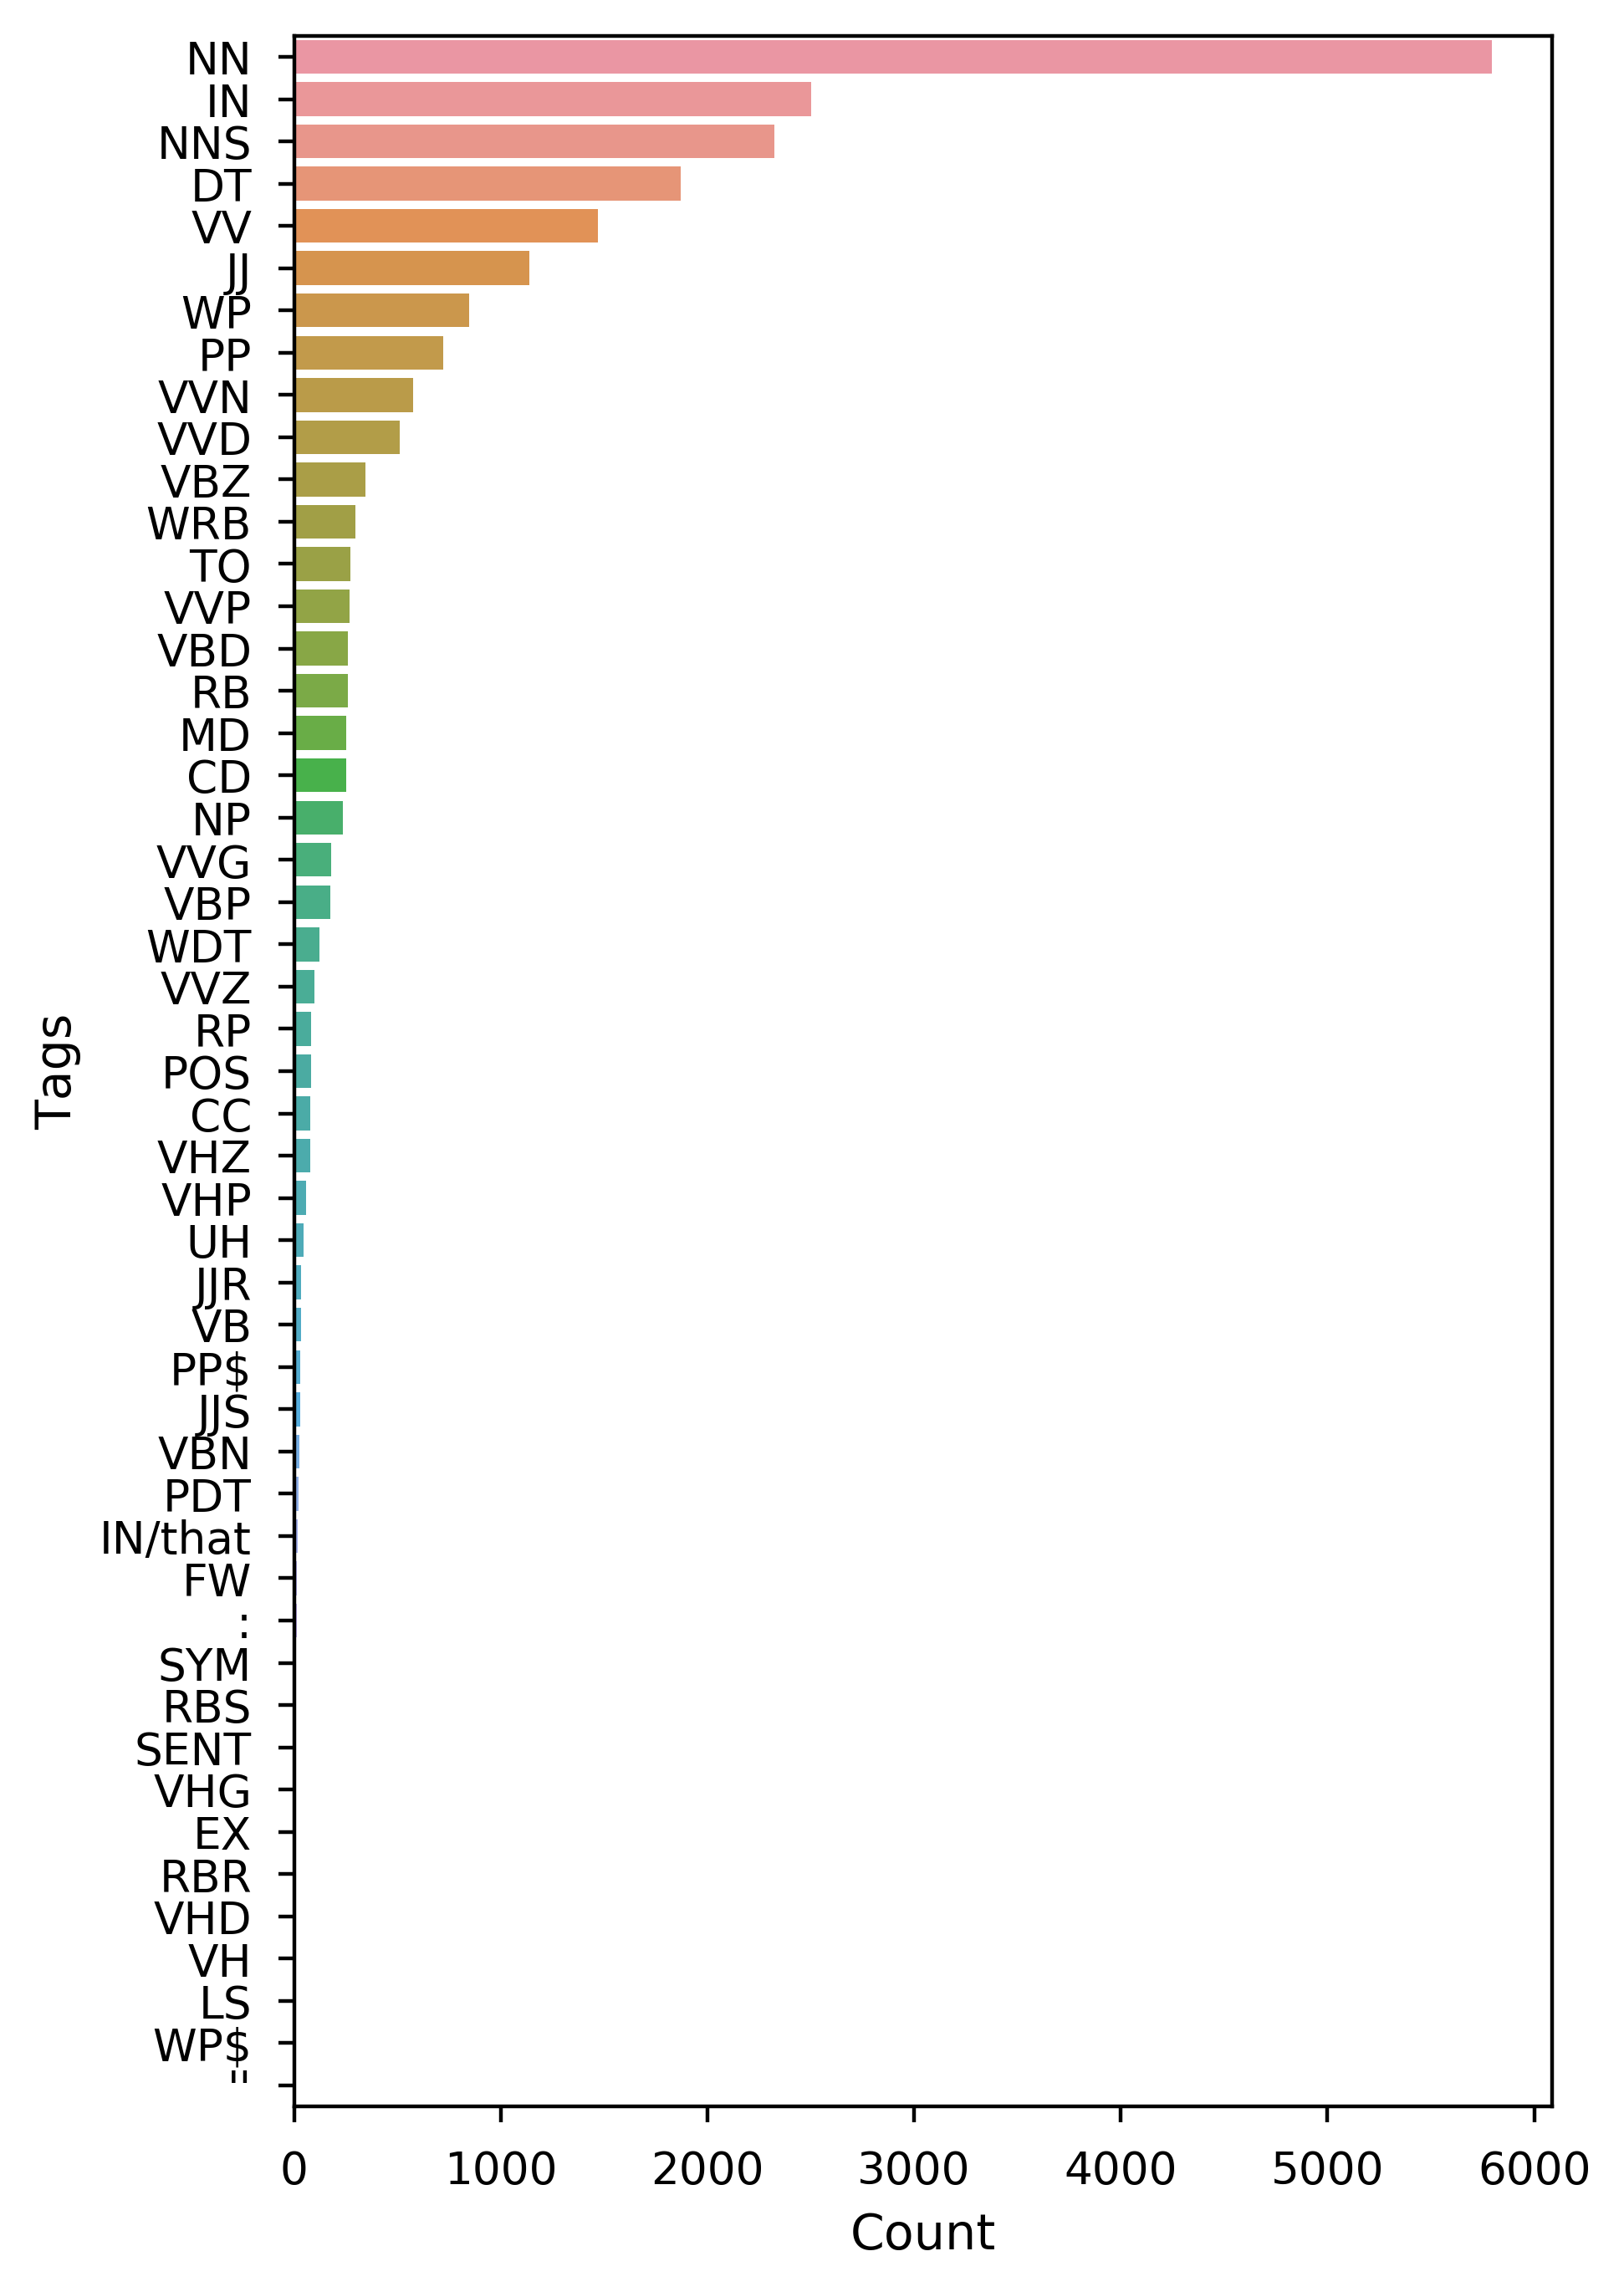
\includegraphics[scale=0.6]{barplot_pos_counts}
	
	Here we can see that most words are actually nouns (by quite a bit), these are the things we're referring to (ie: names of movies, actors, characters). The second most common tag is the \textit{IN} tag which denotes preposition; these tell us the relation between the objects (nouns). Other important tags which appear very frequently are the \textit{WP} and \textit{VV} tags which denote pronouns of the forms \textit{who, what, which} and verbs like \textit{find, show} respectively; this is to be expected considering that the set is composed of queries about the movie domain.

\section{Evaluation}
	
	An "evaluation" pipeline was set up to evaluate the performance of the modes. This consists of running the trained model on the test set and generating a file that holds all the predictions, then the actual metrics are computed with the \textit{Conlleval} script\footnote{The Conlleval script was originally created to evaluate the performance of models for the CoNLL-2000 shared task, but we can also use it to evaluate our models.}, that gives us various metrics (specifically the \textit{accuracy, precision, recall and F1}), but we'll only use the \textit{F1} metric to evaluate the performance.

\subsection{Baseline}

	As said in the \textit{Models} section, the baseline model is just a transducer from word to IOB tag and an unsmoothed, unigram model.
	
	\begin{description}
		\item[Baseline F1 Score:] \textit{57.07}
	\end{description}
	
\subsection{Basic Model}
	
	The IOB model is trained on the training set as it's provided. Multiple models were constructed, one for each combination of n-gram length and smoothing methods. Below is a heatmap with the scores of each combination. The \textit{order} axis represents the n-gram length and the \textit{method} axis the smoothing method used, the value in each cell is the F1 score obtained when evaluating the model's prediction on the test set.
	
	\hspace*{-1cm}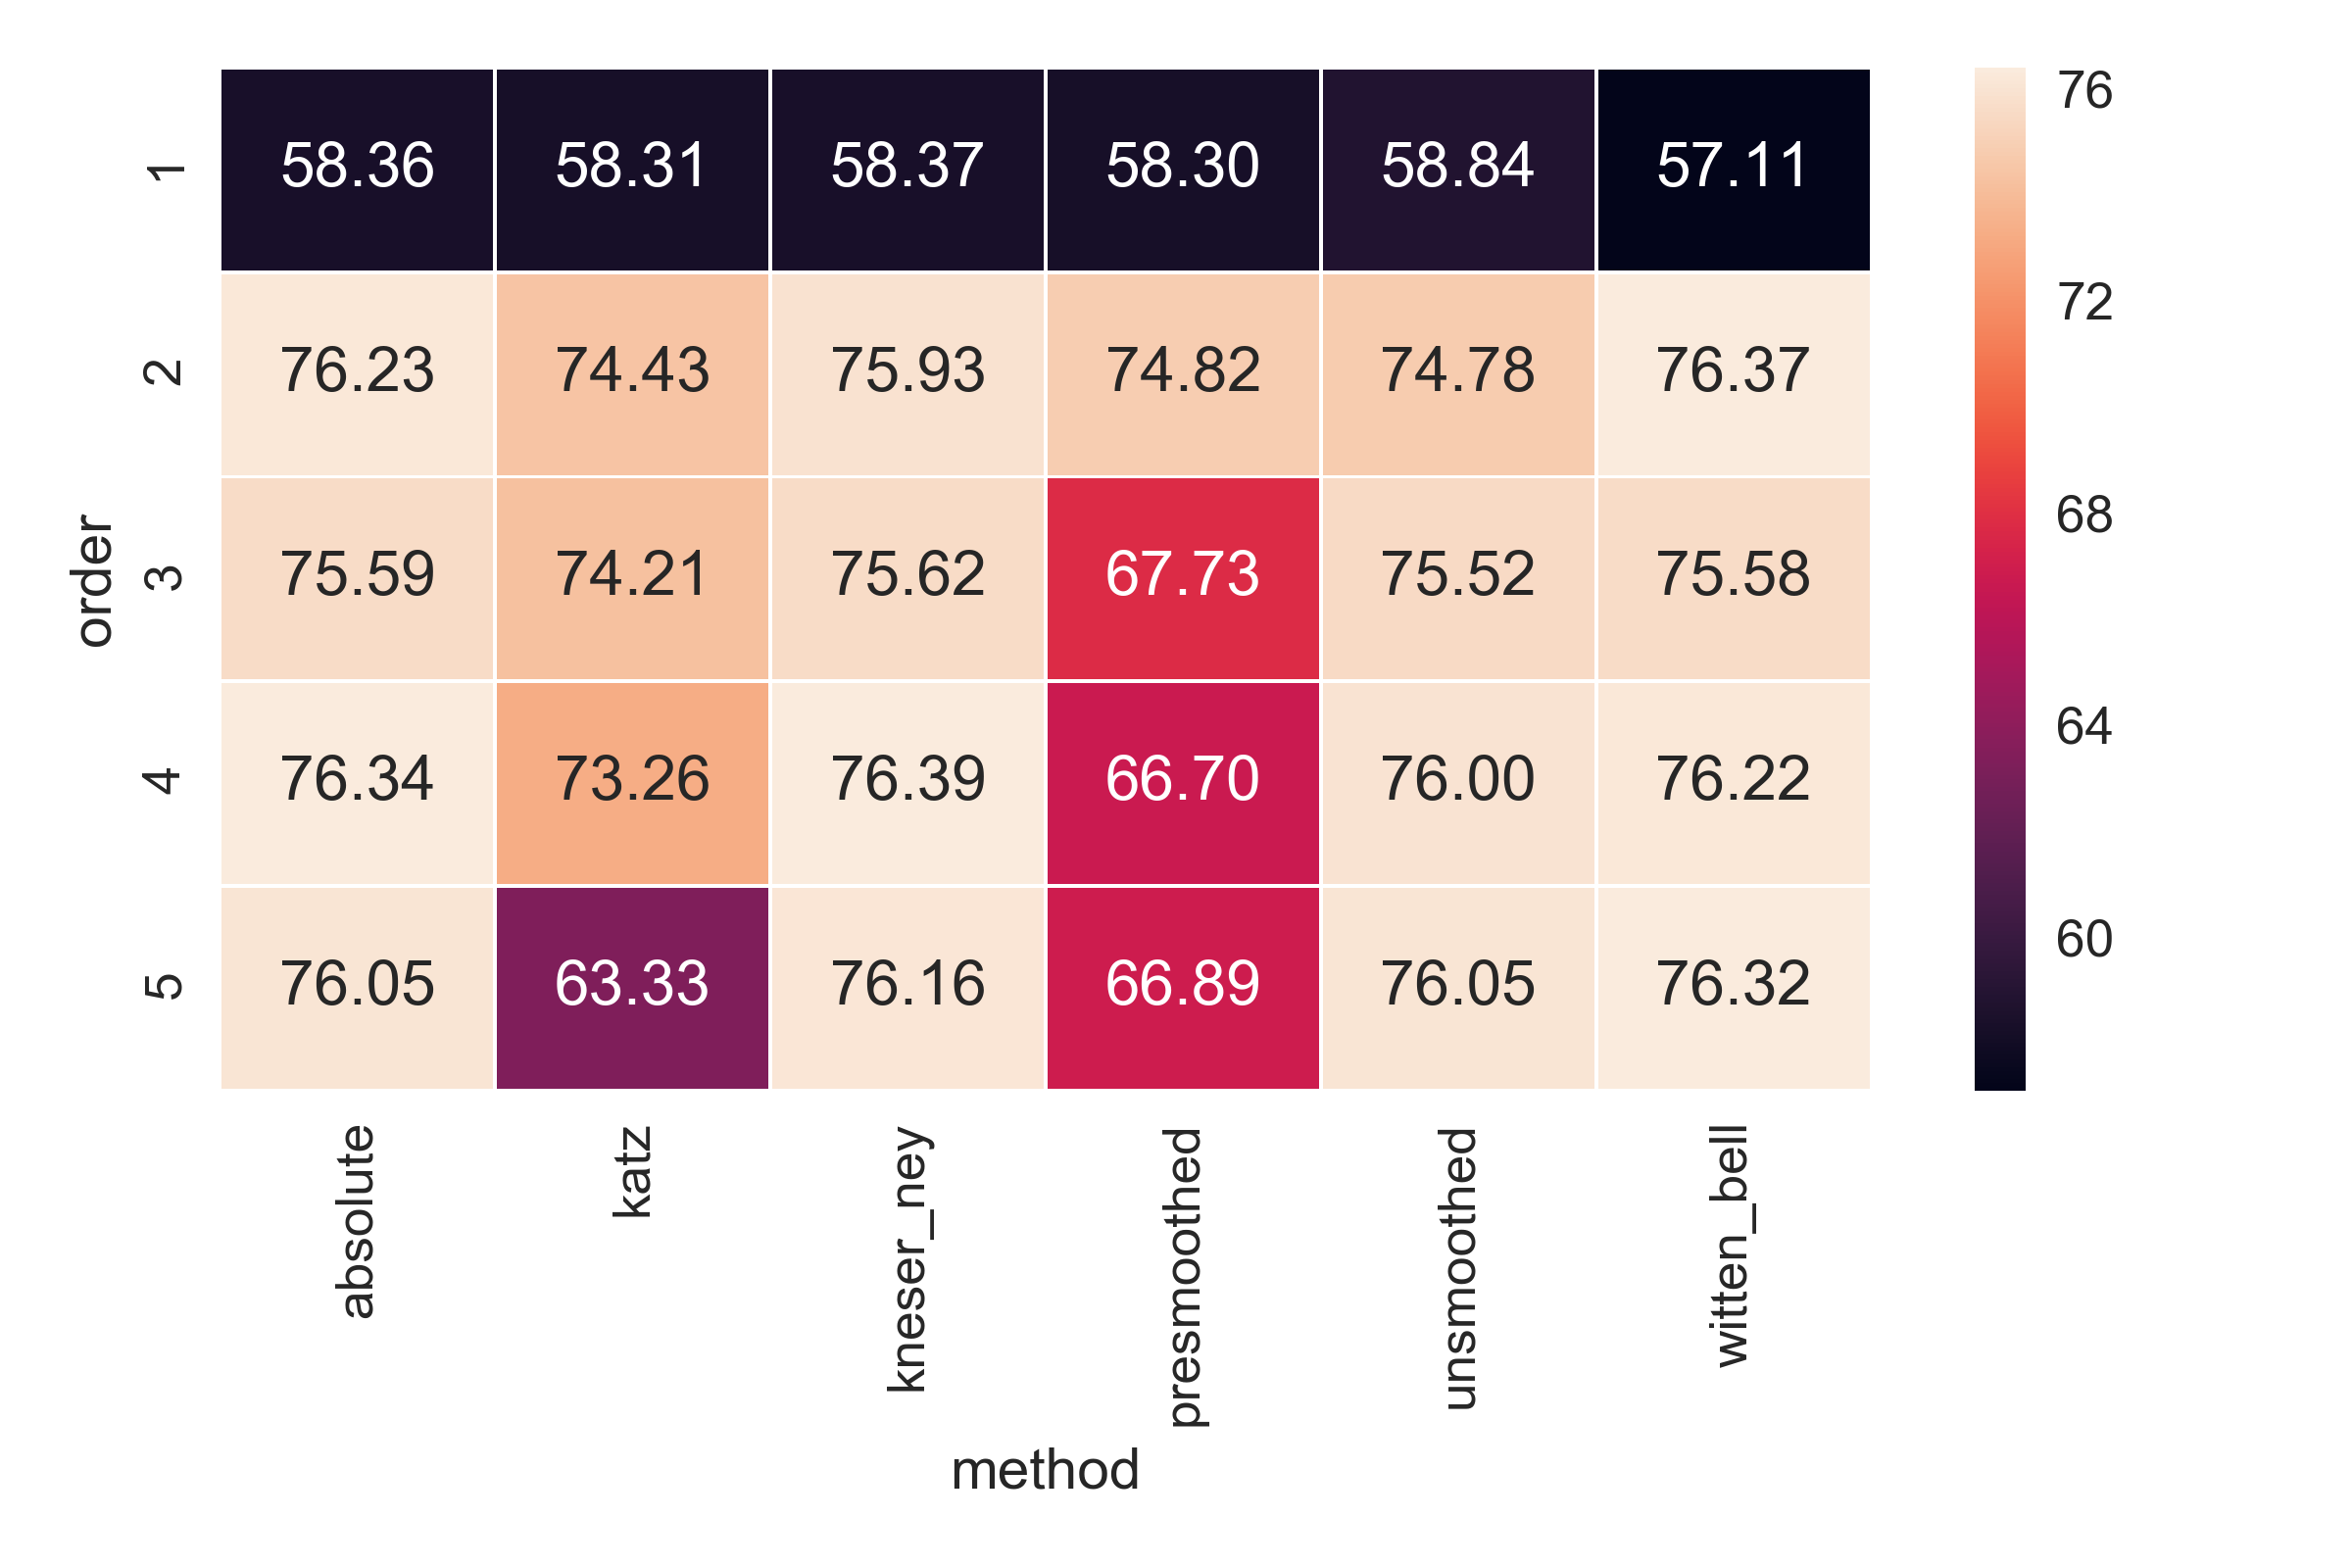
\includegraphics[scale=0.6]{scores_heatmap_w2iob}
	
	As we can see, the model didn't have a very good performance when using a unigram length, but even so these are better than the baseline model. For all other n-gram lengths it seems that the score does not vary so much from one length to the other. There is also no smoothing algorithm that is consistently better than the others, but it seems that for higher n-gram lengths the performance seems to increase. Following are the 3 best F1 scores obtained for the basic model, sorted by F1 score.
	
		
	\begin{table}[h]
		\centering
		\begin{tabularx}{155pt}{l | c | c}

			\textbf{Method} & \textbf{Order} & \textbf{F1 Score} \\
			\hline 
			kneser ney & 4 & 76.39 \\
			\hline
			witten bell & 2 & 76.37 \\
			absolute & 4 & 76.34 \\
			
		\end{tabularx} 
		\caption{Best \textit{Basic Model} F1 Scores}
		\label{table:basic-method-scores}	
	\end{table}
	
		
\subsection{Improved Model}
	
	The improved model was trained on a slightly modified version of the training set. Since plain \textit{O} tags don't give much information to the model about the word they're supposed to 'tag' these have been replaced with \textit{O\_\_word}. Basically the model predicts all tags, except the O ones, in the same way as the basic model, but instead of predicting O tags it now predicts the word per se (replacing \textit{O} with \textit{O\_\_word} is actually the same as replacing \textit{O} with \textit{word}). By doing this simple change we give much information that the model can leverage during prediction. Below is a heatmap of the scores obtained using this improved model:
	
	\hspace*{-0.6cm}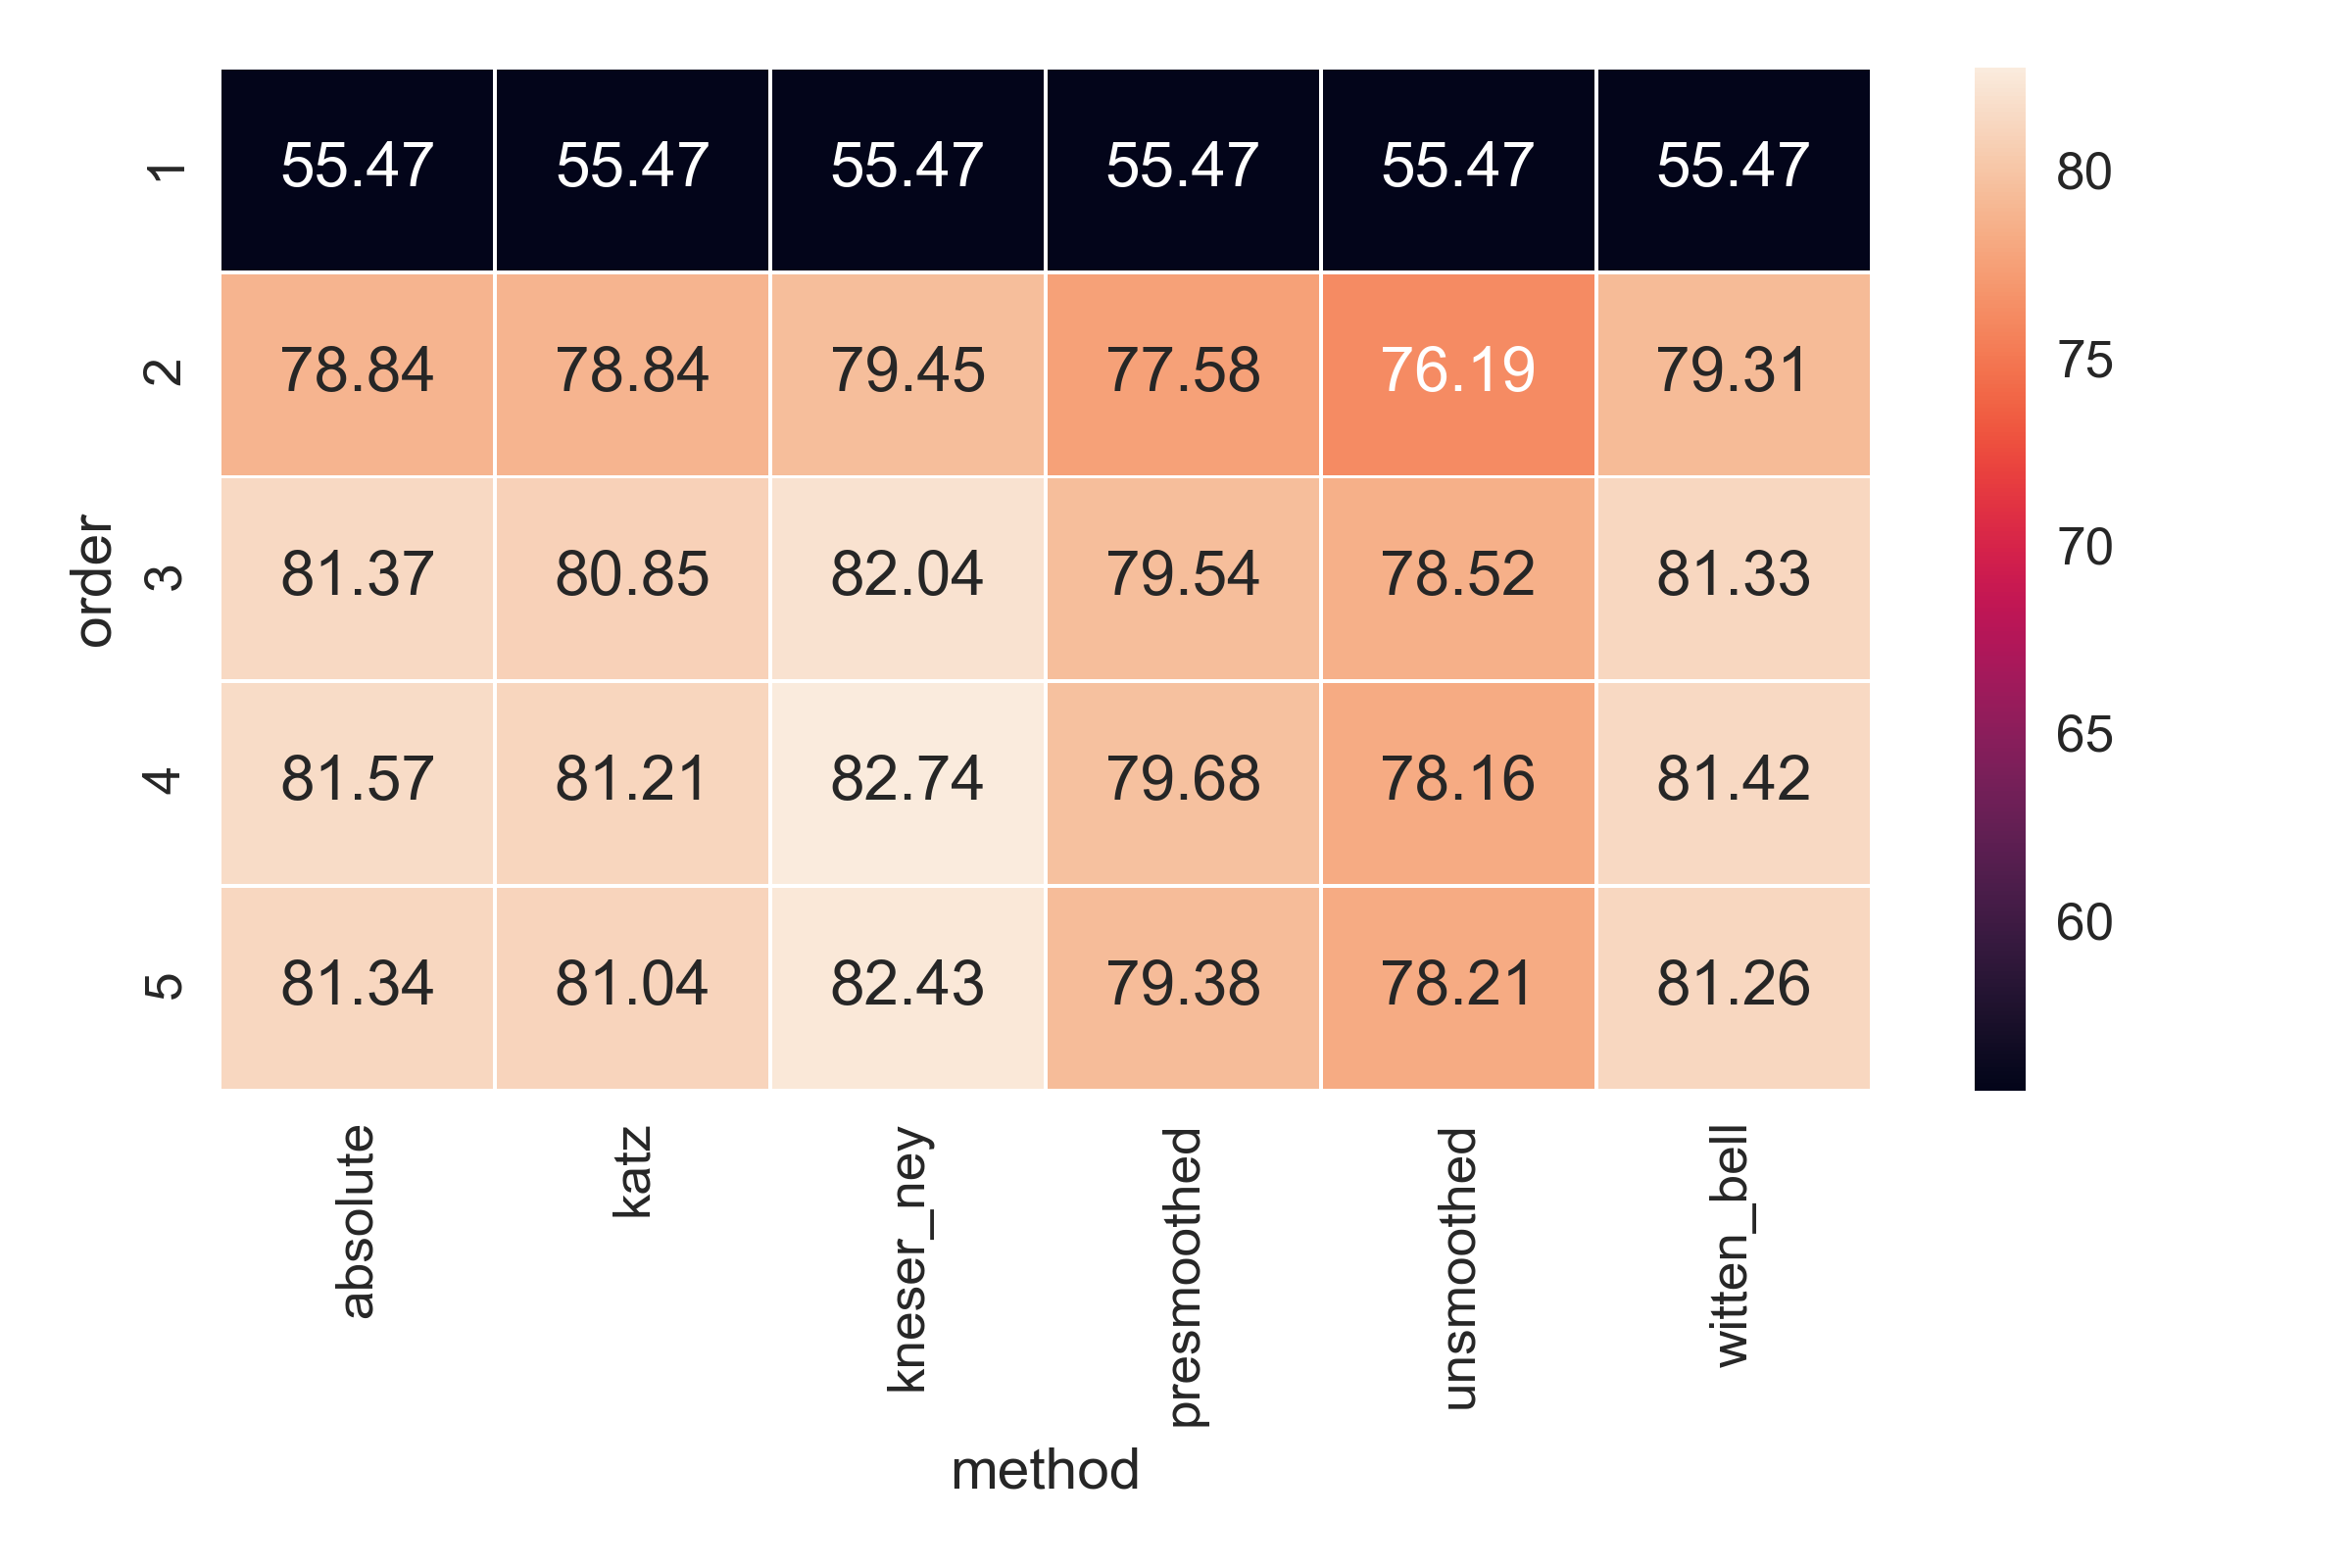
\includegraphics[scale=0.6]{scores_heatmap_w2iob__w}

	If we compare these scores with the basic model's one we can notice that the scores for the unigram length in the improved model are always lower than the ones in the basic model, but all the other scores are higher in the improved model. This makes sense since by replacing the O with O\_\_word we're introducing more complexity in the data, which can only be properly understood by the model if it considers the context in which said new tags appear. Also, by comparing the improved model's scores with the baseline score we can see that all unigram lengths have a lower F1 but every other combination yields a higher one. Below is a table of the combinations which yielded the best F1 score in the improved model:
	
	\begin{table}[h]
		\centering
		\begin{tabularx}{155pt}{l | c | c}

			\textbf{Method} & \textbf{Order} & \textbf{F1 Score} \\
			\hline 
			kneser ney & 4 & 82.74 \\
			\hline
			kneser ney & 5 & 82.43 \\
			kneser ney & 3 & 82.04 \\

		\end{tabularx} 
		\caption{Best \textit{Improved Model} F1 Scores}
		\label{table:improved-method-scores}	
	\end{table}	
			
	An interesting thing to note is that the best combination in both models stayed the same (\textit{kneser ney} and \textit{4}-gram), but the other 2 combinations are different. It seems that in this improved, more complex, model the \textit{kneser ney} method consistently has a better performance for each n-gram length (except for the unigram case in which all scores are the same). By using this improved model we get an improvement of 6.35\% with respect to the basic one.

\section{Future Work}

	For reasons of time or scope there are some other possible improvements we can do to the model that have not been explored in this work. This section will mention some of them in case anyone else is interested in trying them or for future research.
	
	The first possible change that could be worth looking into is mixing in the POS tags with either the words (ie: \textit{word\_\_postag}) or as an extension to the IOB tags (possibly compose them in the same way as we did with \textit{O\_\_word}). This raises the question of how does the performance vary when we add extra information to the words or to the tags. Another thing that might be interesting finding out is if extending the other IOB tags with words as was done with the O tag would increase or decrease the performance of the model. We could also leverage the fact that we have the lemmas in the dataset and try to see if these can be composed with in the words or in the tags either alone or together with the POS tags.
	
	A certain increase in performance could be obtained by transforming our tags from \textit{IOB} format to \textit{BILUO} format (Begin, In, Last, Unit, Out) format, which is as expressive as BIO but has been demonstrated in \cite{DesignChallenges} to be much easier for the model to learn. Even so, it would be interesting to see if extending the O tags in this new format would produce any increase in performance as it did for the IOB one.
	

\section{Conclusion}
	
	In this work we've explored a way in which to build an automatic IOB tagger, train it on some data and predicting the actual tags. We've seen that O tags don't provide much information and the model has a hard time actually learning to differentiate when an O tag is the one that should be predicted and when not. To solve this problem we've added more information to the O tag by extending it with the word it is tagging, in doing so we've practically replaced the O with $\#words$ new tags. After this the model seemed to be able to learn the correct mapping more efficiently.
	
	We've also analyzed various combinations of smoothing methods and n-gram lengths and compared how all their possible combinations affected the final performance of the model. We've seen that for both models the \textit{knesser ney} smoothing together with a \textit{4-gram} underlying model is the combination that works best. In the case of the second model in which we had much more complexity on the \textit{tag} side, \textit{knesser ney} smoothing produced the best 3 results, so it might be that this smoothing method is especially useful when there is high variation in the data (although more research should be done to attest that this is actually the case).



% include your own bib file like this:
\bibliographystyle{plain}
%\bibliography{acl2018}

%\bibliographystyle{plainnat}
\bibliography{acl2018}

%\bibliographystyle{acl_natbib}


\end{document}
